% ==================== 2.3.2.4 NaCl ====================
\jiegou{2.3.2.4}{氯化钠结构（NaCl 型）}

NaCl 结构的演示对象就是 NaCl 本身，它可视作两套面心立方点阵沿 $\langle100\rangle$
方向相互平移 $(1/2,0,0)$ 嵌套而成；建模参数见表~\ref{tab:nacl}。

\begin{table}[H]
  \centering
  \caption{氯化钠（NaCl）结构的建模参数}
  \label{tab:nacl}
  \begin{tabular}{ll}
    \toprule
    项目 & 参数 \\
    \midrule
    空间群 & $F\,m\,\bar3\,m$（No.~225） \\
    晶格常数 & $a=b=c=5.62$\,\AA，$\alpha=\beta=\gamma=90^\circ$ \\
    原子坐标 & Na$^+$：$(1/2,0,0)$（$4b$ 位）；Cl$^-$：$(0,0,0)$（$4a$ 位） \\
    化学式单元数 & $Z=4$ \\
    \bottomrule
  \end{tabular}
\end{table}

\begin{figure}[H]
  \centering
  \subcaptionbox{空间群与晶格常数设置}{%
    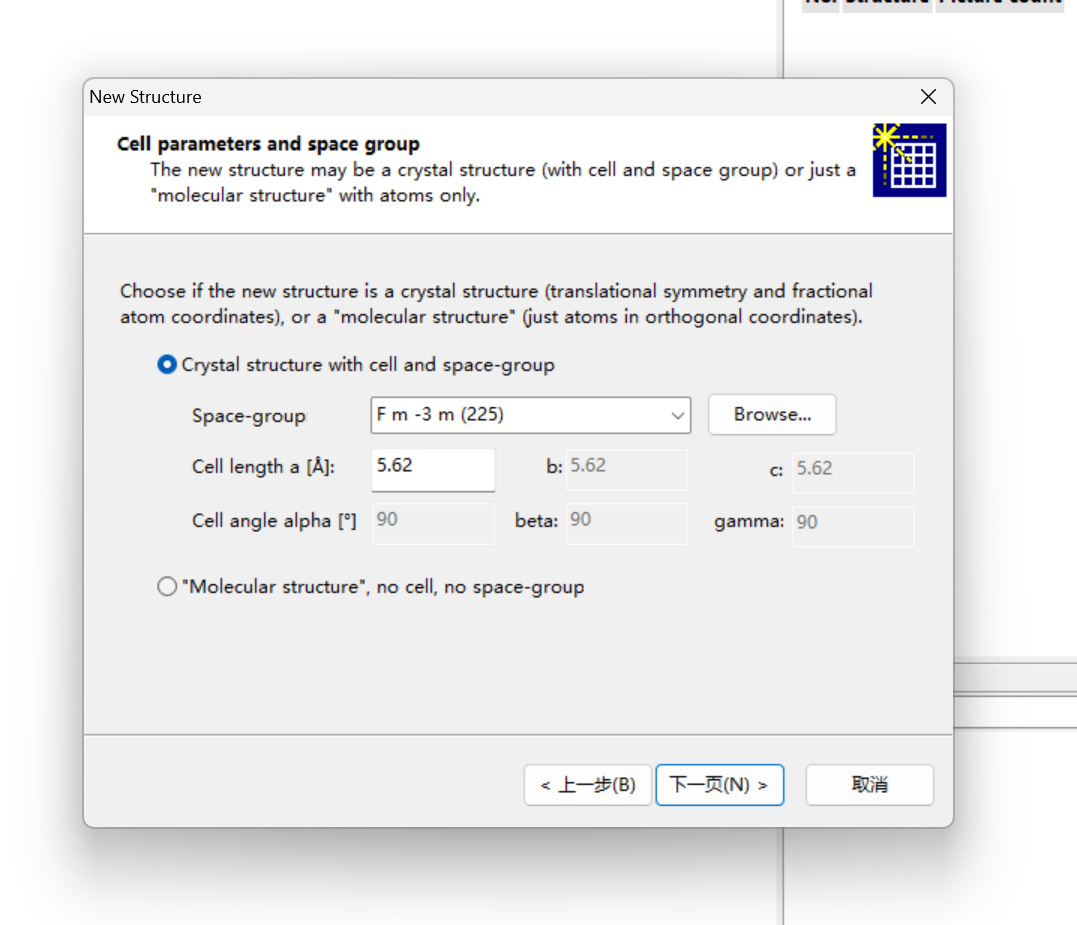
\includegraphics[width=0.44\textwidth]{assets/nacl/a.png}}
  \hfill
  \subcaptionbox{非对称单元原子（Na、Cl）添加}{%
    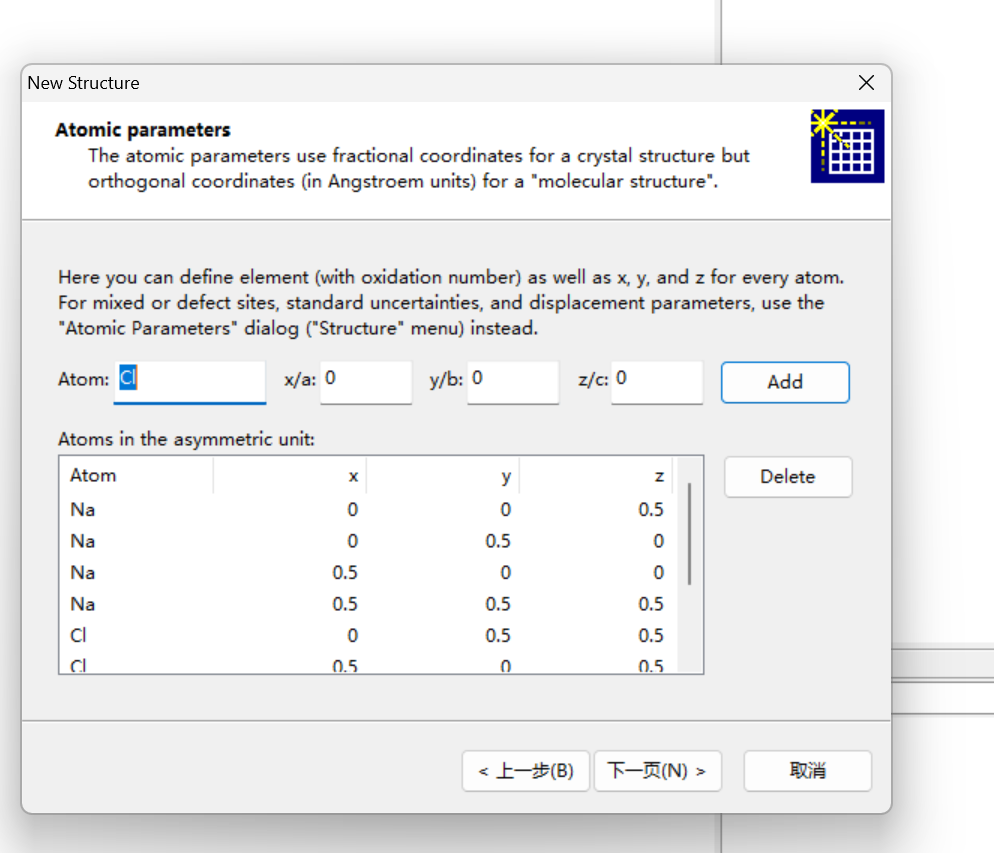
\includegraphics[width=0.44\textwidth]{assets/nacl/b.png}}
  \caption{氯化钠（NaCl）结构的参数设置}
  \label{fig:nacl-param}
\end{figure}

\begin{figure}[H]
  \centering
  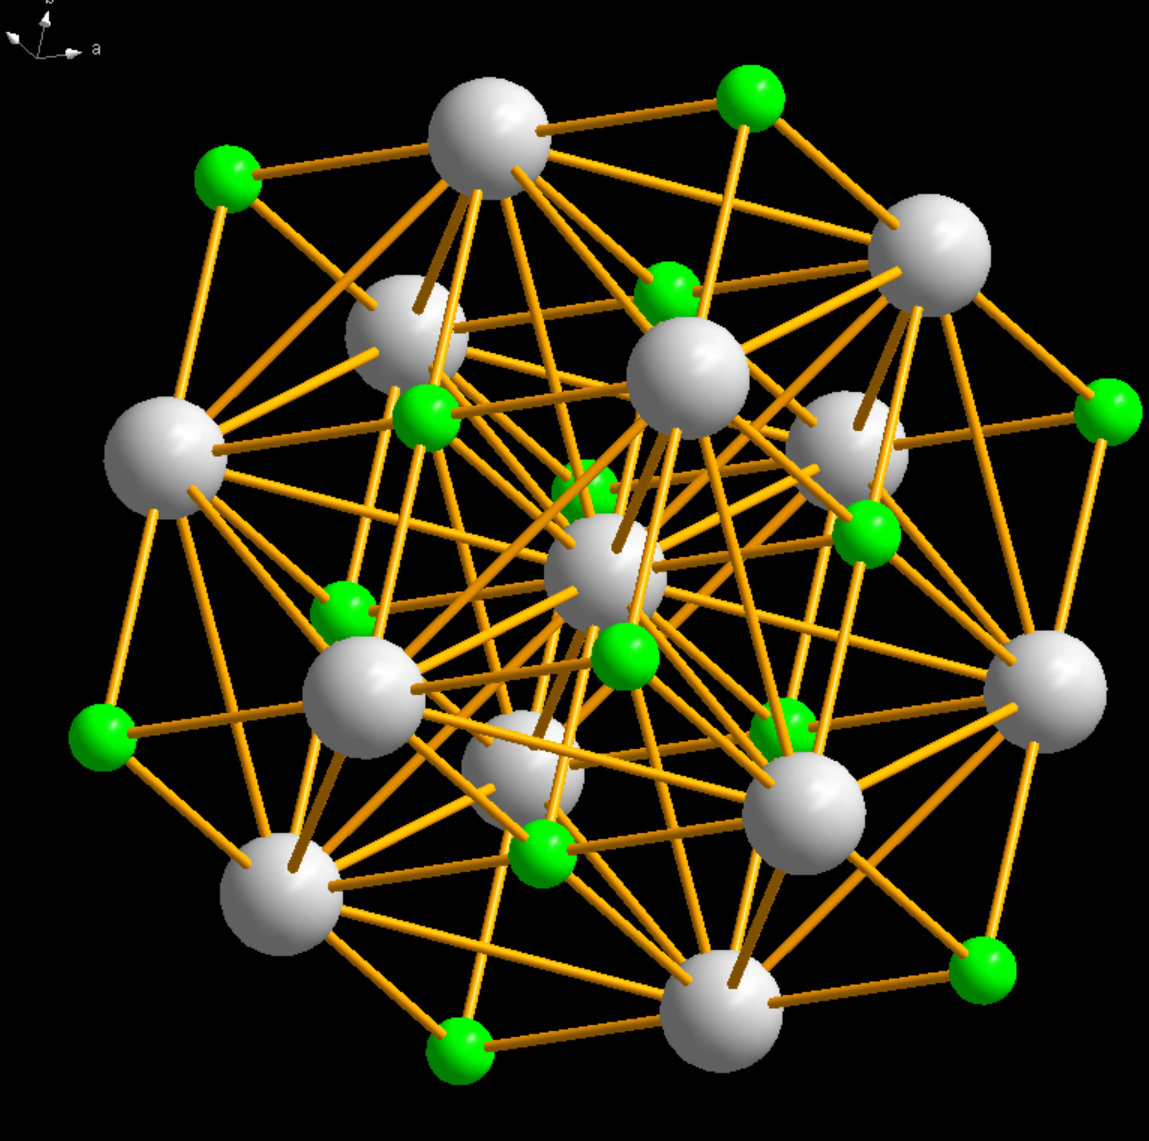
\includegraphics[width=0.5\textwidth]{assets/nacl/c.png}
  \caption{氯化钠（NaCl）结构的晶体结构模型}
  \label{fig:nacl-model}
\end{figure}

\begin{figure}[H]
  \centering
  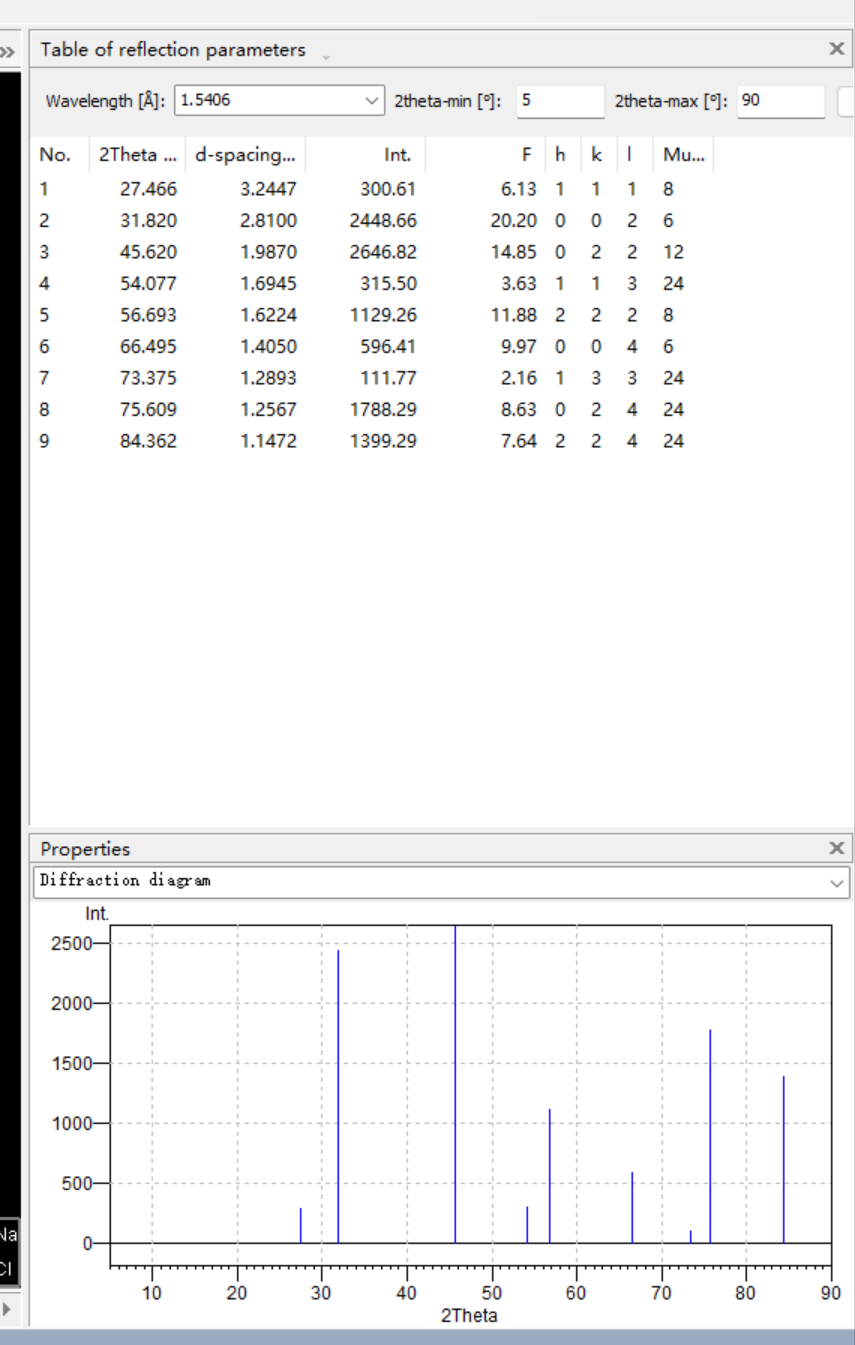
\includegraphics[width=0.4\textwidth]{assets/nacl/d.png}
  \caption{Diamond 模拟的氯化钠（NaCl）结构粉末衍射图}
  \label{fig:nacl-xrd}
\end{figure}

\begin{figure}[H]
  \centering
  \subcaptionbox{密排晶面视图}{%
    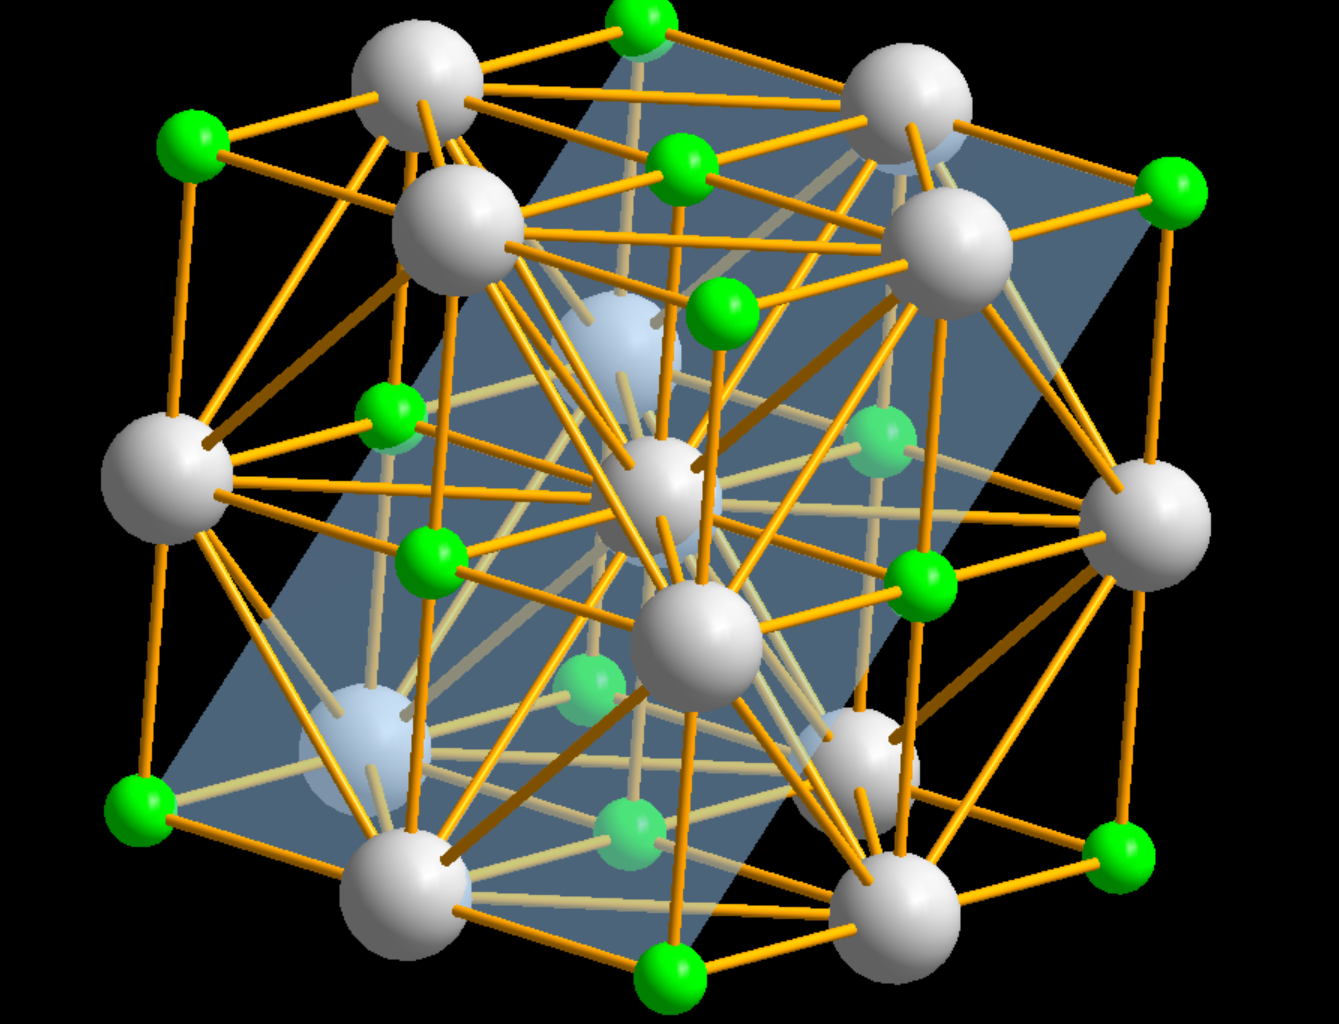
\includegraphics[width=0.40\textwidth]{assets/nacl/e.png}}
  \hfill
  \subcaptionbox{配位八面体（配位数 6）}{%
    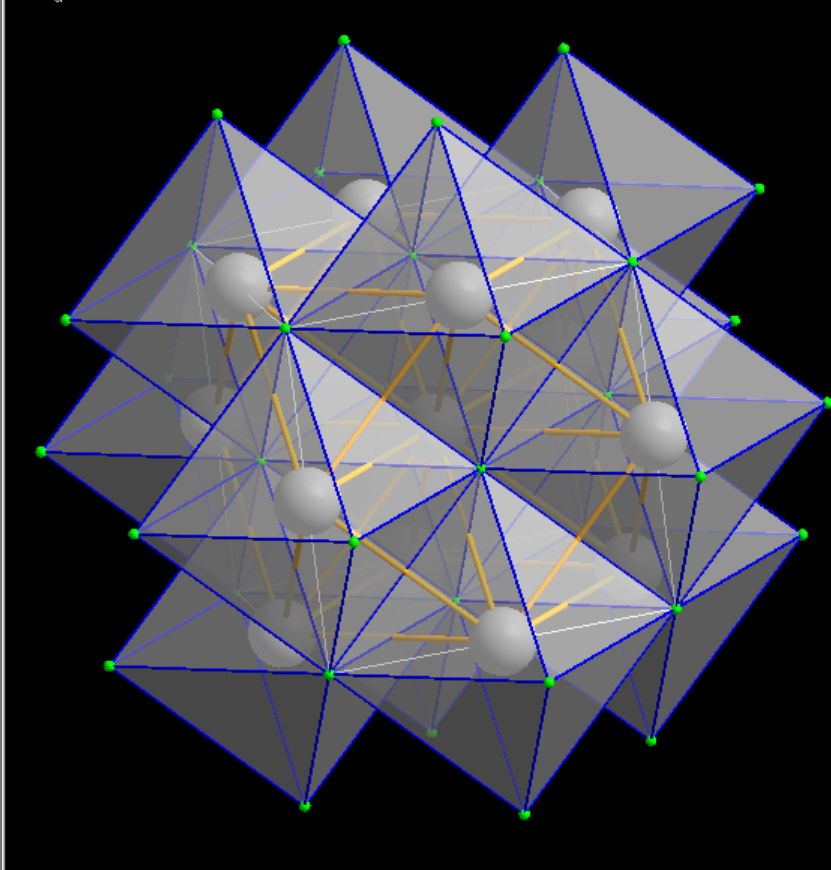
\includegraphics[width=0.28\textwidth]{assets/nacl/f.png}}
  \hfill
  \subcaptionbox{配位多面体设置}{%
    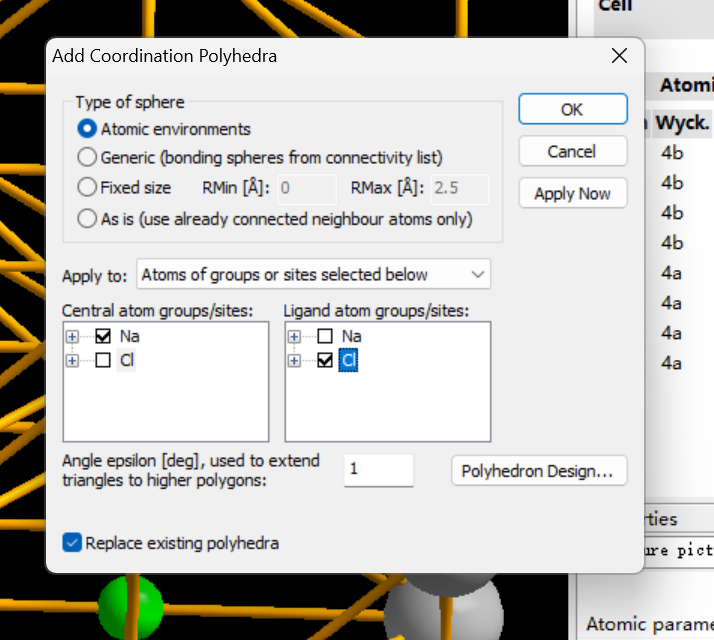
\includegraphics[width=0.24\textwidth]{assets/nacl/f1.png}}
  \caption{氯化钠（NaCl）结构的晶面与配位八面体}
  \label{fig:nacl-plane}
\end{figure}

\textbf{两套亚格子。}从图~\ref{fig:nacl-model} 可以看到 Na$^+$ 与 Cl$^-$ 沿晶胞棱方向
交替排列：Cl$^-$ 占顶点与面心，构成一套 FCC 点阵；Na$^+$ 占各棱中点与体心，相当于
另一套沿 $\langle100\rangle$ 平移 $a/2$ 的 FCC 点阵。两套亚格子叠加后，晶胞内有
4 个 Na$^+$ 与 4 个 Cl$^-$，即 4 个 NaCl 化学式单元。

两种离子的配位数都是 6，配位多面体为正八面体（图~\ref{fig:nacl-plane}(b)），Na--Cl
距离 $d=a/2=2.81$\,\AA。离子半径比 $r_+/r_-\approx0.54$ 落在八面体（六配位）的稳定
范围 $0.414\sim0.732$ 之内，与结构观察一致。再借助晶格常数计算理论密度：
\begin{equation}
  \rho=\frac{ZM}{N_Aa^3}
    =\frac{4\times58.44\ \mathrm{g/mol}}{6.022\times10^{23}\times
      (5.62\times10^{-8})^3\ \mathrm{cm^3}}
    \approx2.19\ \mathrm{g/cm^3}
\end{equation}
与实测密度（约 $2.16$ g/cm$^3$）接近，实际晶体中的缺陷使密度略低于理论值。KCl、LiF
等碱金属卤化物和 MgO、CaO、FeO 等氧化物都采取 NaCl 型结构。
